\chapter{Design And Implementation}
% - Design and Implementation
%   - overview
%   - original tinkering and considerations
%   - features and considerations
%       - readline
%       - golang
%       - logging
%       - extensibility
%       - embedded files
%           - Running examples
%           - syscalls (combined output)
%       - usability 
%   - architecture of cli-tool
%   - architecture of web-tool
%       - how sandboxing is achieved
\label{chap:design}
\section{Overview}
% Libs and tools used

\section{Architecture}
\section{Extending CLI-Tutor}

\begin{lstlisting}[float=htbp, frame=single, language={}, label=lst:markdown, caption=Specification for Markdown lesson files.]
# Lesson Title

A line under a level 1 heading is the lesson description. This is also
displayed in the menu.

## First Task Title

Task instructions are parsed as normal lines under a level 2 heading.

Even line breaks and nested elements will reflect in the lesson. This greatly
enhances readability.

`Commands` are highlighted with backticks.

Text can be injected into a lesson at the time of parsing with template
functions like this --> {{SomeFunc}}

## Second Task Title

This is the first line following a second level 2 heading and thus the text of
task #2.

```
Code blocks can also be used to represent larger blocks of instructions or for
ASCII diagrams.
```
## Interactive tasks with expected values

If the current task is expecting a certain output to a command the user types,
we can specify that using the `>` syntax.

> {{TestFunc}}

## Runtime expected value calculation

Sometimes the correct value for a given task can only be computed at run time,
to achieve this we can specify the expected value of a task to be the output of
a system call by prepending a `!` and then the expected command.

> !ls -la

### Lesson Vocabulary (Provided as a comma separated list of values under a
level 3 heading )

vim, ls, cp, cat, echo <--- only these commands will be permitted in this lesson.

\end{lstlisting}

\subsubsection{Subsubsection}

\paragraph{Paragraph.} Always with a point.


\begin{figure}[htbp]
	\centering
	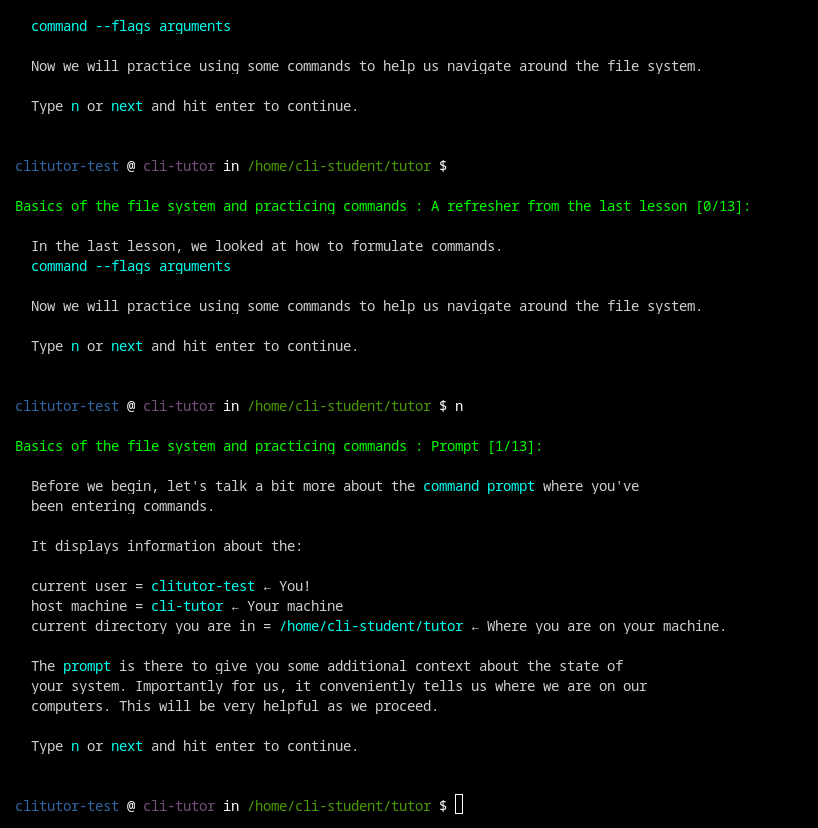
\includegraphics[width=1\textwidth]{img/cliexpansionfull}
	\caption{Screen shot of a \textit{CLI-Tutor} lesson showing values interpolated into the lesson.}
	\label{fig:templateexpansion}
\end{figure}
